\documentclass{exam}
\usepackage{ulem}
\usepackage{xcolor}
\usepackage{amsmath}
\usepackage{amssymb}
\usepackage{mathtools}
\usepackage{commath}
\usepackage{derivative}

\usepackage[lmargin=71pt, tmargin=1.2in]{geometry}  %For centering solution box
\usepackage{tikz}
\usetikzlibrary{mindmap}

\lhead{Analisi II - Domande teoriche\\}
\rhead{Enrico Barbuio\\}
% \chead{\hline} % Un-comment to draw line below header
\thispagestyle{empty}   %For removing header/footer from page 1

\newcommand{\R}[0]{\mathbb{R}}
\newcommand{\N}[0]{\mathbb{N}}
\newcommand{\err}[1]{\textcolor{red}{#1}}
\newcommand{\nota}[1]{\textcolor{blue}{\textbf{Nota: }#1}}

%\pointsdroppedatright
\printanswers
\renewcommand{\solutiontitle}{\noindent\textbf{Sol:}\enspace}   % answer keyword

\begin{document}
% header
\begingroup  
    \centering
    \LARGE Analisi II\\
    \LARGE Domande teoriche\\[0.5em]
    \large \today\\[0.5em]
    \large Prof. Davide Guidetti\par
    \large Svolgimento Enrico Barbuio\par
    \large Fisica - Unibo - A.A. 2024/2025\par
\endgroup
\par\noindent\rule{\textwidth}{0.4pt}

\section*{Spazi metrici}
\begin{questions}

\question Dare la definizione di spazio normato. Darne un esempio e dimostrare che effettivamente lo e’.
\begin{solution}
    Uno spazio normato è una coppia ordinata $(X, \norm{\cdot})$ con $X$ spazio vettoriale e $\norm{\cdot}$ norma. La norma è una funzione $X \xrightarrow{} [0, + \infty[$ t.c. 
    \begin{enumerate}
        \item $\forall  x \in X, \forall \lambda \in \mathbb{K} \quad \norm{\lambda x} = \abs{\lambda} \norm{x}$
        \item $\forall x \in X, \forall y \in X \quad \norm{x+y} \leq \norm{x} + \norm{y}$
        \item $x \in X, \quad \norm{x} = 0 \Rightarrow x=0$
    \end{enumerate}
    Esempio: $X = \R^n, \norm{x} \coloneqq \sum_{i=0}^n\abs{x_i}$, infatti:
    \begin{enumerate}
        \item $\norm{\lambda x} = \sum_{i=0}^n\abs{\lambda x_i} = \sum_{i=0}^n\abs{\lambda} \abs{x_i} = \abs{\lambda} \sum_{i=0}^n\abs{x_i} = \abs{\lambda} \norm{x}$
        \item $\norm{x+y} = \sum_{i=0}^n\abs{x_i + y_i} \leq \sum_{i=0}^n(\abs{x_i} + \abs{y_i}) = \norm{x} + \norm{y}$
        \item $\norm{x} = 0 \iff \sum_{i=0}^n\abs{x_i} = 0 \iff  x_i = 0$
    \end{enumerate}
\end{solution}

\question Mostrare come si puo’ definire una norma su uno spazio con prodotto interno. Dare un esempio.
\begin{solution}
    Siano $(X, < \ldots , \ldots>)$ s.v. e prodotto interno. Per $x \in X$ definisco $\norm{x} \coloneqq \sqrt{<x,x>}$.\\
    Per esempio posti: $X = \R^n, \quad <x,y> = \sum_{i=0}^n x_i y_i$, 
    la norma sarà quella euclidea: $\norm{x} = (\sum_{i=0}^n x_i^2)^{1/2}$
\end{solution}

\question Definire la norma della convergenza uniforme in $BC(A)$ ($A$ insieme). Provare che con questa norma, la convergenza puntuale di una successione equivale alla convergenza uniforme.
\begin{solution}
    Ricordo che $BC(A)$ è lo spazio vettoriale delle funzioni $f: A \rightarrow \R $ continue e limitate. Su questo spazio possiamo definire la norma come segue: $\norm{f}_{BC(A)} = \sup_{a \in A} \abs{f(a)}$.
    \err{magari intendeva "\sout{con questa norma}" "in questo spazio"?} quindi sarebbe prop 2.5\\
    FAI DIM!!!
\end{solution}

\question Dare la definizione di spazio metrico e presentare, illustrandolo, un esempio.
\begin{solution}
    Uno spazio metrico è una coppia ordinata $(X,d)$ con $X$ insieme e $d$ metrica. Una metrica è una funzione $d: X \times X \rightarrow [0,+\infty[$ t.c.
    \begin{enumerate}
        \item $\forall x, y \in X \quad d(x,y) = d(y,x)$ \quad (proprietà commutativa)
        \item $\forall x,y,z, \in X \quad d(x,y) \leq d(x,z) + d(z,y)$ \quad (disuguaglianza triangolare)
        \item $\forall x, y \in X \quad d(x,y)=0 \iff x=y$
    \end{enumerate}
    Per esempio $X = \R^n $ con la metrica associata alla norma: $d(x,y) \coloneqq \norm{x-y}$.\\
    \dots verifica proprietà \dots (facile)
\end{solution}
\nota{norma definita su s.v., metrica su semplice insieme}

\question Dare la definizione di interno di un sottoinsieme e di sottoinsieme aperto in uno spazio metrico. Dimostrare che l’intersezione di due aperti e’ un aperto.
\begin{solution}
    Sia $(X,d)$ uno spazio metrico e $A\subseteq X$ un suo sottoinsieme. L'interno di $A$ è $\mathring{A} \coloneqq \{x \in A \ |\ \exists \  r >0 : B(x,r) \cap X \subseteq A\} $.
    $A$ è un sottoinseme aperto se $A=\mathring{A}$.\\
    Siano $A_1, A_2$ sottoinsiemi aperti di $X$, allora $A_1 \cap A_2$ è un aperto.\\
    Infatti: $\forall x \in A_1 \cap A_2 \quad \exists\  r_1,r_2 : B(x,r_1) \cap X \subseteq A_1, B(x,r_2) \subseteq A_2$,\\
    scelto $r=\min\{r_1, r_2\}$ ho che $B(x,r)\subseteq B(x,r_1) \subseteq A_1$ e $B(x,r)\subseteq B(x,r_2) \subseteq A_2$.
\end{solution}

\question Dare la definizione di frontiera di $A$ sottoinsieme di uno spazio metrico e presentare, illustrandolo, un esempio.
\begin{solution}
    Sia $A$ sottoinsieme aperto di uno spazio metrico $X$.
    La frontiera di $A$: $Fr(A)$ è l'insieme delle $x\in X \ : \ \forall r>0, B(x,r)$ contiene sia elementi di $A$ che del suo coniugato.
    
    Ad esempio siano $X = \R^2$ e $A=\{(x,y) \in \R^2 \ | \ x^2+y^2 \leq 1, \ x>0\}$. 
    $Fr(A) = [(0,-1), (0,1)] \cup \{ (x,y) \in \R^2 \ | \ x^2+y^2 =1, \ x\geq0 \}$
\end{solution}

\question Dare la definizione di frontiera di $A$ sottoinsieme di uno spazio metrico e dimostrare che, se $A \subseteq X$, con $X$ spazio metrico, $A$ e’ aperto se e solo se $A \cap Fr(A) = \emptyset $.
\begin{solution}
    Sia $A$ sottoinsieme aperto di uno spazio metrico $X$.
    La frontiera di $A$: $Fr(A)$ è l'insieme delle $x\in X \ : \ \forall r>0, B(x,r)$ contiene sia elementi di $A$ che del suo coniugato.
    
    Ricordo la definizione di aperto: $A$ è aperto se $A = \mathring{A}=\{x \in A \ | \ \exists \ r>0 : B(x,r) \subseteq A\}$.\\ 
    ($\Longrightarrow$) Se $x \in A$ con $A$ aperto, allora $\exists \ r>0 : B(x,r) \subseteq A$, perciò $\exists \ r>0 : B(x,r) \cap (X \setminus A) = \emptyset$
    quindi $x \not\in Fr(A)$ $\Longrightarrow A\cap Fr(A) = \emptyset$.\\
    ($\Longleftarrow$) Che $ \mathring{A} \subseteq A$ è ovvio. Dimostro che $A \subseteq \mathring{A}$:\\
    $\forall x \in A, \ x \not\in Fr(A) \quad\Longrightarrow\quad \forall x \in A,\  \exists\  r>0 : $ o $B(x,r) \subseteq A$ o $B(x,r) \subseteq (X\setminus A)$.
    Ma la seconda condizione non si può verificare in quanto sicuramente $x \not\in X \setminus A$ quindi deve essere che $B(x,r) \subseteq A$ quindi $x \in \mathring{A}$
\end{solution}

\question Sia $A \subseteq X$ spazio metrico. Scrivere cosa significa che $A$ e’ chiuso. Provare che $A$ e’ chiuso se e solo se $X \setminus A$ e’ aperto.
\begin{solution}
    $A$ si dice chiuso se $Fr(A) \subseteq A$.

    Osservo che $Fr(A) = Fr(X \setminus A)$. Inoltre so che: $A$ è aperto $\iff$ $A \cap Fr(A) = \emptyset$\\
    $Fr(A) \subseteq A \quad \iff \quad Fr(A) \not\subseteq X \setminus A \quad \iff \quad Fr(X \setminus A) \not\subseteq X \setminus A \quad\iff\quad X\setminus A \not\subseteq \mathring{(X\setminus A)}$
\end{solution}

\question Dare la definizione di chiusura $\overline{A}$ di $A$, con $\overline{A} \subseteq X$ spazio metrico. Dimostrare che $x_0 \in A$ se e solo se esiste una successione a valori in $A$ convergente a $x_0$.
\begin{solution}
    La chiusura di $A$ è l'insieme: $\overline{A} \coloneqq A \cup Fr(A)$

    $x_0 \in A \quad\iff\quad \exists\  \{a_n\}_{n \in N} \subseteq A \ : \ d(a_n,x_0) \xrightarrow{n \rightarrow +\infty} 0$
    
    ($\Longrightarrow$) se $x_0 \in A$ scelgo $a_k = x ,\ \forall k\in\N$\\
    se $x_o \in Fr(A)\setminus A$ so che $\forall r>0,\  B(x_0,r)\cap A \not= \emptyset$. Scelgo $a_k \in B(x_0, \frac{1}{k})\cap A$ e ho che $d(a_k,x_0)\leq \frac{1}{k} \xrightarrow{k\rightarrow + \infty} 0 \quad\Longrightarrow\quad a_k \xrightarrow{k\rightarrow + \infty}x_0$
    
    
    ($\Longleftarrow$) \textbf{RAA:} se $x_0 \not\in \overline{A}$ allora $\exists r>0 : B(x_0, r) \cap A = \emptyset$. Dato che $\{a_k\} \subseteq A$, $\exists \epsilon > 0 : \forall k, \  d(a_k,x_0) >\epsilon \quad \Longrightarrow \quad a_k\not \longrightarrow x_0$\\
    \nota{dim prof diversa:}
    Se $x_0 \in A$ ho fatto.\\
    Se $x_0\not\in A$ : $\forall r>0,\ \exists n(r) >0 : k> n(r) \Rightarrow a_k \in B(x_0,r)\cap A \not= \emptyset $ inoltre $\{x_0\} \in B(x_0, r)\setminus A \not= \emptyset$ $\quad\Longrightarrow\quad x_0 \in Fr(A)$
\end{solution}

\question Dare la definizione di limite di una successione in uno spazio metrico. Provare che se il limite esiste, è unico.
\begin{solution}
    Sia $(X, d)$ s.m., $\{x_k\}_{k\in \N}$ successione. $x_n$ ha per limite $l\in X$ ($\lim_{n\rightarrow + \infty} x_n = l$) se $\forall \epsilon>0, \exists N>0 : k>N \Rightarrow d(x_n, l) < \epsilon$

    Siano $l,m \in X : x_n \rightarrow l$ e $x_n \rightarrow m$\\
    $\forall \eta, \exists n_1(\eta),n_2(\eta) \quad:\quad n< n_1(\eta) \Rightarrow  d(x_n,l) < \epsilon $ e $ n< n_2(\eta) \Rightarrow d(x_n,m)< \epsilon$\\
    $d(l,m) < d(l, x_n) + d(x_n, m) < 2\eta$ se $ n> N = \max\{n_1(\eta),n_2{\eta}\}$\\
    da cui $d(l,m) = 0  \quad\Longrightarrow \quad l=m$
\end{solution}

\question Sia $A \subseteq X$ spazio metrico. Dare la definizione di punto di accumulazione di $A$. Dare un esempio di punto di accumulazione appartenente ad $A$ e uno di punto di accumulazione non appartenente ad $A$.
\begin{solution}
    $x\in X$ è punto di accumulazione di $A$ ($x \in D(A)$) se $\forall r>0, B(x,r) \cap A \setminus \{x\} \not= \emptyset$

    Esempi:
    \begin{equation*}
        A \coloneqq \{x=\frac{1}{n}:n \in \N\}, x= 0.\quad  x \not\in A, x \in D(A)
    \end{equation*}
    \begin{equation*}
        A \coloneqq \R, x= 0.\quad  x \in A, x \in D(A)
    \end{equation*}
\end{solution}

\question Dare la definizione dell'espressione $\lim_{x\rightarrow x_0} f(x) = l$, con $f: A \subseteq X \rightarrow Y$ e $X$, $Y$ spazi metrici, illustrandola con un esempio. Provare che, se $f$ è continua in $x_0$ e $\lim_{n\rightarrow + \infty}a_n = x_0$ ($a_n \in A$), allora $\lim_{n\rightarrow + \infty} f(a_n) = l$ ed, eventualmente, il viceversa.
\begin{solution}
$\lim_{x\rightarrow x_0} f(x) = l$ se $ \forall\epsilon, \exists \delta(\epsilon) : x \in A \cap B(x_0, \delta(\epsilon)) \setminus \{x_0\} \Rightarrow d_Y(f(x),l)<\epsilon$.

Esempio $f(x) = (0,x)$, $\lim_{x\rightarrow 0} f(x)=(0,0)$.

\err{continua}
\end{solution}

\question Sia $f: A \rightarrow \R^n$, con $A\subseteq X$ spazio metrico. Illustrare il legame tra il limite della funzione per $a \rightarrow x_0$ e il limite delle componenti. Dove deve stare $x_0$?
\begin{solution}
    Affinché il limite abbia senso è necessario che $x_0 \in D(A)$ altrimenti $\exists r>0 : A\cap B(x_0,r) = \emptyset$.

    $\lim_{a\rightarrow x_0}f(a) = l \quad \iff \quad \forall i \in n \ \lim_{a\rightarrow x_0}f_i(a) = l_i $
\end{solution}

\question Illustrare cosa si può dire sui limiti di restrizioni. 
\begin{solution}
    Ricordo la definizione di restrizione: sia $A\subseteq B\subseteq X$ s.m., $f:B\to Y$, la restrizione di $f$ ad $A$ è la funzione $f\restriction_A: A \to Y \ : \ \forall x \in A, f\restriction_A(x) = f(x)$
    
    Proprietà:
    \begin{itemize}
        \item Se $x_0 \in D(A)$ e $\lim_{x \to x_0} f(x) = l$ allora $\lim_{x \to x_0} f\restriction_A (x) = l$
        \item Se $\lim_{x \to x_0} f\restriction_A (x) = l$ e $\exists r>0 \ : \ B(x_0,r) \cap B \subseteq A$ allora $\lim_{x \to x_0} f(x) = l$
    \end{itemize}
\end{solution}

\question Dare la definizione di $f$ continua in $a_0$ , con $f: A \rightarrow Y$ , $A \subseteq X$, $X , Y$ spazi metrici. Descrivere la connessione tra questa definizione e quella di limite.
\begin{solution}
    $a_0 \in A \err{\cap D(A)}$ , $f$ continua in $a_0$ se $\forall \epsilon > 0 \ \exists \delta(\epsilon)>0 \ :\  x \in B(a_0,\delta(\epsilon)) \cap A \Rightarrow d(f(x), f(a_0))<\epsilon$ 

    \begin{itemize}
        \item Se $a_0 \in A \setminus D(A)$ allora $f$ è continua in $a_0$
        \item Se $a_0 \in A \cap D(A)$ allora $f$ è continua in $a_0$ se e solo se $\exists \lim_{x\to a_0} f(x) = f(a_0)$
    \end{itemize}
\end{solution}

\question Enunciare ed, eventualmente, dimostrare un teorema di continuità per composizioni di funzioni continue.
\begin{solution}
    Siano $X,Y,Z$ s.m., $f: A \subseteq X \to Y$ e $g: B \subseteq Y \to Z$ continue, con $f(a) \subseteq B$. Se $f$ continua in $x_0$ e $g$ continua in $f(x_0)$ allora $g \circ f$ è continua in $x_0$.

    \textbf{Dim:} fissato $\epsilon>0$, dalla continuità di $g$ ho che:
    $\exists r(\epsilon)>0 \ : \ y \in B_Y(f(x_0), r(\epsilon)) \cap B \Rightarrow d(g(y), g(f(x_0)) < \epsilon$\\
    dalla continuità di $f$ ho che $\exists \delta = \delta(r(\epsilon)) > 0 \ : \ x \in B_X(x_0, \delta)\cap A \Rightarrow d(f(x), f(x_0))< \epsilon$\\
    per cui se $x \in B_X(x_0, \delta)\cap A$ allora $d(g \circ f(x), g \circ f(x_0))< \epsilon$.
\end{solution}

\question Dare la definizione di sottoinsieme limitato in uno spazio metrico. Caratterizzare i sottoinsiemi limitati negli spazi normati.
\begin{solution}
    Sia $A\subseteq X$ s.m., $A$ è limitato se $\delta(A)<\infty$.\\
    $\delta(A)$ è il diametro di $A$ ossia $\sup_{a_0,a_1 \in A} \{d(a_0,a_1)\}$
    
    \err{???}
\end{solution}

\question Dare la definizione di sottoinsieme compatto di uno spazio metrico. Illustrare la connessione tra ”compattezza” e ”chiusura e limitatezza”.
\begin{solution}
    Sia $A\subseteq X$ s.m., $A$ è compatto se ogni successione a valori in $A$ ammette una sottosuccessione con convergente in $A$.

    Se $A$ è compatto allora è anche chiuso e limitato ma in generale non vale viceversa. \err{controesempio?}

    Se $X = \R^n$ allora vale anche il viceversa. \err{dim?}
\end{solution}

\question Enunciare ed, eventualmente, dimostrare (anche parzialmente) qualche versione del teorema di Weierstrass negli spazi metrici.
\begin{solution}
    Sia $A\subseteq X$ compatto, $f: A \to Y$ continua.
    Allora: $f(A)$ è compatto e se $Y=\R$ allora $f$ ammette $\max$ e $\min$

    \err{DIM!!!}
    \end{solution}

\question Dare la definizione di funzione uniformemente continua nell'ambito degli spazi metrici e in quest'ambito enunciare, ed eventualmente dimostrare, una versione del teorema di Heine-Cantor.
\begin{solution}
    Sia $f: A\subseteq X \rightarrow Y$ con $X$ e $Y$ s.m., $f$ è uniformemente continua se $\forall \epsilon>0,  \exists \delta(\epsilon)>0 \ : \ \forall x_0,x_1 \in A$ con $ d(x_0,x_1)<\delta(\epsilon),\ d(f(x_0), f(x_1)) <\epsilon$.

    H-C: se $A$ è compatto, $f\in C(A,Y) \Longrightarrow f \in UC(A,Y)$\\
    \err{DIM!!!}
\end{solution}

\question Illustrare le nozioni di sottoinsieme convesso di uno spazio vettoriale e di sottoinsieme connesso per archi in uno spazio metrico. Illustrare qualche connessione tra esse. 

\question Illustrare ed, eventualmente, dimostrare qualche versione del teorema di Bolzano negli spazi metrici.

\question Dare la definizione di successione di Cauchy in uno spazio metrico e di spazio metrico completo. Presentare un esempio di spazio metrico completo e un esempio di spazio metrico che non lo e’.

\question Dare le definizioni di sottoinsieme chiuso di uno spazio metrico e di spazio metrico completo. Dimostrare che un sottoinsieme chiuso di uno spazio metrico completo e’ completo.

\question Enunciare ed eventualmente dimostrare il teorema delle contrazioni, specificando il significato di ogni termine che compare in esso.
    
\end{questions}

\section*{Integrali di superficie, formule di Gauss-Green e di Stokes}

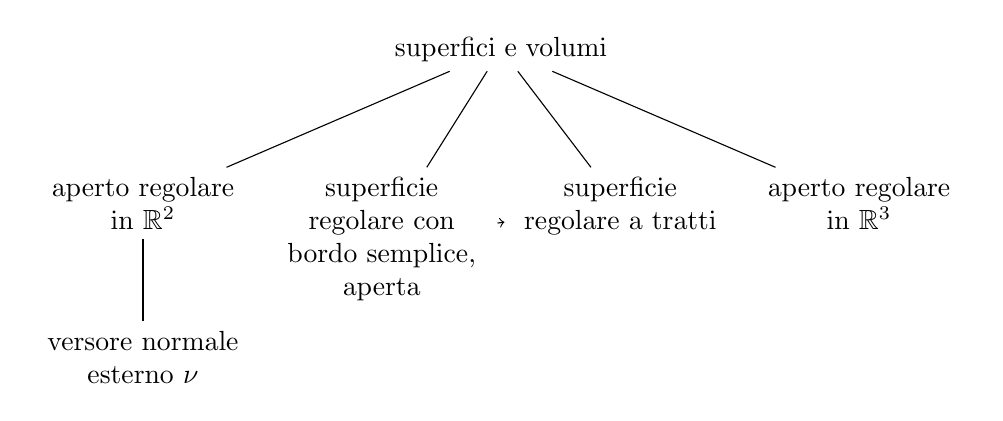
\begin{tikzpicture}
    [text width=\linewidth/4.5, align=flush center, anchor=north,
    level/.style={sibling distance=\linewidth/4}]
    
\node{superfici e volumi}
    child {
        node {aperto regolare in $\R^2$}
        child { node {versore normale esterno $\nu$}}
        }
    child { node (supaperta) {superficie regolare con bordo semplice, aperta}}
    child { node (suptratti) {superficie regolare a tratti}}
    child { node {aperto regolare in $\R^3$}};
    \draw[->] (supaperta) -- (suptratti);
\end{tikzpicture}

\begin{questions}
\question Dare la definizione di aperto regolare in $\R^2$, assieme a quelle delle varie nozioni che intervengono in essa.
\begin{solution}
    Sia $\Omega$ un aperto in $\R^2$, $\Omega$ è un aperto regolare se:
    \begin{enumerate}
        \item è limitato e connesso per archi
        \item $Fr(\Omega)$ è unione di una famiglia finita di sostegni di cammini $\gamma^1 ,\dotsc, \gamma^p$ regolari e tali che:
        $1\leq i < j \leq p$,  $\gamma^i$ e $\gamma^j$ si intersecano al più negli estremi
        \item $\forall x \in \Omega, \exists r<0 \quad : \quad B(x,r) \setminus Fr(\Omega) = A_1 \cup A_2$ con $A_1 \subseteq \Omega$ e $A_2 \cap \Omega = \emptyset$
    \end{enumerate}

    $A\subseteq \R^n$ è limitato se: $\delta(A) < + \infty$, con $\delta(A)$ diametro di $A$ $\coloneqq\sup\{d(x_1,x_2) | \forall x_1, x_2 \in A\}$

    $A\subseteq \R^n$ è connesso per archi se: $\forall x, y \in A, \exists \phi:[a,b] \to R^n$ cammino continuo, con $\phi([a,b])\subseteq A$ e $\phi(a) = x,\  \phi(b) = y$.

    $\gamma$ cammino regolare se: è $C^1$, semplice e con $\gamma'(t) \not= 0 \ \forall t$. Per semplice si intende che $\gamma\restriction_{]a,b]}$ e $\gamma\restriction_{[a,b[}$ sono iniettive.
\end{solution}

\question Enunciare le formule di Gauss-Green in $\R^2$ . Precisare la nozione di versore normale esterno.
\question Definire e illustrare la nozione di prodotto vettoriale in R3 .
\question Dare la definizione di superficie regolare, con bordo, semplice, aperta; di bordo e di superficie regolare a tratti. Mostrare un esempio.
\question Dare la definizione di area e di integrale per una superficie regolare con bordo semplice, aperta e per una superficie regolare a tratti.

\begin{solution}
Sia $S$ una superficie regolare, con bordo, semplice, aperta e $(\Phi, \Omega)$ una sua parametrizzazione.

L'area di $S$ vale $\int_S d\sigma = \int_{\overline{\Omega}} \norm{\pdv{\Phi}{\theta} \times \pdv{\Phi}{\phi}} d\theta d\phi$.

Sia $f: S \to \R$, l'integrale di superficie di $f$ su $S$ vale: $\int_{S}f(x) d\sigma = \int_{\overline{\Omega}} f(\Phi(\theta, \phi)\norm{\pdv{\Phi}{\theta} \times \pdv{\Phi}{\phi}} d\theta d\phi$, qualora la funzione sia sommabile.

Se invece $S$ è una superficie regolare a tratti con $S_j$, per $j=1 ,\dots, p $ superficie regolare, con bordo, semplice, aperta tale che $S = \cup_{j=1}^p S_j$ come da definizione.
Allora $\int_S d\sigma = \sum_{j=1}^p \int_{S_j} d\sigma$ e $\int_S f(x) d\sigma = \sum_{j=1}^p \int_{S_j} f(x) d\sigma$ qualora $f$ sia integrabile su ogni $S_j$.
\end{solution}

\question Dare la definizione di versore normale e di orientamento per una superficie regolare con bordo semplice, aperta. Mostrare che esistono esattamente due orientamenti.
\question Dare la definizione di aperto regolare in $\R^3$ e di versore normale esterno.

\begin{solution}
    Sia $\Omega$ un aperto in $\R^3$. $\Omega$ è regolare se:
    \begin{enumerate}
        \item è limitato e connesso per archi.
        \item $Fr(\Omega) = \cup_{j=1}^p S_j$, con $S_j$ superficie regolare, con bordo, semplice, aperta.
        \item $i \not= j \ \Longrightarrow\  S_i \cap S_j = \partial S_i \cap \partial S_j$.
        \item $\forall x \in Fr(\Omega), \ \exists r>0 \ : \ B(x,r) \setminus Fr(\Omega) = U_1 \cup U_2$ con $U_1, U_2$ limitati e connessi per archi e tali che $U_1 \subseteq \Omega$ e $U_2 \cap \Omega = \emptyset$
    \end{enumerate}

\err{
Siano $\Omega$ e $S_j$ come appena definiti. Per $j=1,\dots,p$ definisco versore normale esterno a $\Omega$ l'orientamento su $S_j$ tale che $\forall x \in S_j \setminus \partial S_j, \ \exists t>0 \ : \ \forall s \in [0,t[ \ \  x+s\nu^j \not\in \Omega$.
}
\end{solution}

\question Enunciare le formule di Gauss-Green in $\R^3$. Ricavare da esse il teorema della divergenza.

\begin{solution}
    Sia $\Omega$ un aperto regolare in $\R^3$, $f\in C^1(\overline{\Omega})$, $S_j$ come da definizione di aperto regolare e $\nu^j$ i rispettivi versori normali esterni. 
    \[
    \int_{\overline{\Omega}} \pdv{f}{x_i} dx = \sum_{j=1}^p\int_{s_j} f(x) \nu^j_i d \sigma
    \]
    
    Sia inoltre $U\subseteq \R^3$ aperto connesso per archi con $\Omega \subseteq U$ e $F \in C^1(U; \R^3)$ un campo vettoriale. Allora:
    \[ 
    \int_{\overline{\Omega}} \nabla \cdot F(x) dx = \sum_{i=1}^3 \int_{\overline{\Omega}} \pdv{F_i}{x_i} (x) dx = \sum_{i=1}^3 \sum_{j=1}^p \int_{s_j}F_i \nu^j_i d \sigma = \sum_{j=1}^p \int_{S_j} F \cdot \nu^i d\sigma
    \]
\end{solution}
\question Enunciare la formula di Stokes. Presentare un esempio.
\begin{solution}
    Sia $U$ aperto connesso per archi in $\R^3$ e $F\in C^1(U;\R^3)$.
    Sia poi $S \subseteq U$ una superficie regolare con bordo semplice, aperta e $\nu$ un suo orientamento.
    Siano infine $\eta^j$ cammini regolari che \err{orientano positivamente $\partial S$}.
    \[
    \int_S \nabla \times F (x)\cdot\nu(x)  d\sigma = \sum_{j=1}^p \int F \cdot d\eta^j 
    \]
\end{solution}    
\end{questions}
\end{document}